\documentclass[10pt,letterpaper,twocolumn]{article}
\usepackage[utf8]{inputenc}
\usepackage{amsmath}
\usepackage{amsfonts}
\usepackage{amssymb}
\usepackage{graphicx}
\usepackage{footnote}
\usepackage{float}
\usepackage{booktabs}
\usepackage{subfigure}
\usepackage{multirow}
\usepackage{tabularx} 
\usepackage{url}
\usepackage{caption}
\captionsetup[figure]{skip=0pt} 
\usepackage{siunitx} % Para habilitar el símbolo de ohmios (Ω)
\usepackage{listings}
\lstset{language=Python}
\usepackage{tikz}
\usepackage{circuitikz}
\DeclareSIUnit{\angstrom}{\textup{\AA}}
\DeclareGraphicsExtensions{.bmp,.png,.pdf,.jpg,.eps}
\usepackage[spanish,activeacute]{babel}
%M�rgenes
\usepackage{vmargin}
\setmargins
{10mm}            % margen izquierdo
{1.5cm}           % margen superior
{190mm}           % anchura del texto
{23.42cm}         % altura del texto
{10pt}            % altura de los encabezados
{1cm}             % espacio entre el texto y los encabezados
{0pt}             % altura del pie de p�gina
{1cm}             % espacio entre el texto y el pie de p�gina


\title{\noindent\\[-4cm]\bfseries Experimento N°1}
\author{Felipe Halabi
\\\small\itshape \textit{Departamento de física, Universidad Nacional Andrés Bello, Santiago, Chile}
\\\small\itshape Física Computacional de la Materia}

\date{24 de Septiembre 2024}

\date{26 de Abril 2024}

\begin{document}
\renewcommand{\tablename}{Tabla}
\twocolumn[
\begin{@twocolumnfalse}
\maketitle
\begin{abstract}
El objetivo de este experimento es estudiar la interacción de los átomos para una celda del 
gas noble Xenon, en el cual se analizara el comportamiento de la temperatura, energía cinética, 
energía potencial, distribución de átomos y el número de coordinación a través de simulaciones 
computacionales en el software Las Palmeras Molecular Dynamics (LPMD).

\vspace{5mm}

\end{abstract}
\end{@twocolumnfalse}
\noindent\
]
\section*{Introducción}
El Xenón (Xe) es un elemento químico perteneciente al grupo de los gases nobles, con número 
atómico 54. Es un gas incoloro, inodoro, y no reactivo en condiciones normales, conocido por 
su estabilidad química y su baja reactividad debido a su configuración electrónica completa. 
A diferencia de otros gases nobles más ligeros como el helio, el xenón puede formar algunos 
compuestos en condiciones extremas debido a su mayor número de electrones y su capacidad para 
expandir su capa de valencia.

El Xenón cristaliza en estructuras cúbicas centradas en las caras (FCC) a bajas temperaturas, 
lo que significa que en estado sólido sus átomos están dispuestos en una red en la que cada 
átomo tiene 12 vecinos más cercanos, en una disposición de alta simetría y densidad empacada.

\begin{figure}[h!]
    \centering
    \usetikzlibrary{3d,calc,backgrounds}

\pgfdeclarefunctionalshading{sphere}{\pgfpoint{-25bp}{-25bp}}{\pgfpoint{25bp}{25bp}}{}{
%% calculate unit coordinates
25 div exch
25 div exch
%% copy stack
2 copy 
%% compute -z^2 of the current position 
dup mul exch
dup mul add
1.0 sub
%% and the -z^2 of the light source 
0.3 dup mul
-0.5 dup mul add
1.0 sub
%% now their sqrt product
mul abs sqrt
%% and the sum product of the rest
exch 0.3 mul add
exch -0.5 mul add
%% max(dotprod,0)
dup abs add 2.0 div 
%% matte-ify
0.6 mul 0.4 add
%% currently there is just one number in the stack.
%% we need three corresponding to the RGB values
dup
0.4
}

\definecolor{verde}{HTML}{adda79}
\definecolor{naranjo}{HTML}{f38d70}

\begin{tikzpicture}[line width=1pt]

  \pgfdeclarelayer{background}
  \pgfsetlayers{background,main}

  \begin{scope}[canvas is xy plane at z=0]
    \draw[fill=black!10,opacity=0.5] (0,0) -- (0:2) -- ([turn]90:2) -- ([turn]90:2) -- cycle;
  \end{scope}
  \begin{scope}[canvas is xy plane at z=2]
    \draw[fill=black!10,opacity=0.5] (0,0) -- (0:2) -- ([turn]90:2) -- ([turn]90:2) -- cycle;
  \end{scope}
  \begin{scope}[canvas is zx plane at y=0]
    \draw[fill=black!10,opacity=0.5] (0,0) coordinate (E) -- (0:2) coordinate (F) -- 
      ([turn]90:2) coordinate (G) -- ([turn]90:2) coordinate(H) -- cycle;
    \global\coordinate (GE) at (E);
    \global\coordinate (GF) at (F);
    \global\coordinate (GG) at (G);
    \global\coordinate (GH) at (H);
  \end{scope}
  \begin{scope}[canvas is zx plane at y=2]
    \draw[fill=black!10,opacity=0.5] (0,0) coordinate (A) -- (0:2) coordinate (B) -- 
      ([turn]90:2) coordinate (C) -- ([turn]90:2) coordinate (D) -- cycle;
    \global\coordinate (GA) at (A);
    \global\coordinate (GB) at (B);
    \global\coordinate (GC) at (C);
    \global\coordinate (GD) at (D);
  \end{scope}

  \shade[ball color=verde] (GC) circle [radius=2mm];
  \shade[ball color=verde] (GB) circle [radius=2mm];
  \shade[ball color=verde] (GF) circle [radius=2mm];
  \shade[ball color=verde] (GG) circle [radius=2mm];
  \shade[ball color=naranjo] ($(GA)!0.5!(GC)$) circle [radius=2mm];
  \shade[ball color=naranjo] ($(GB)!0.5!(GG)$) circle [radius=2mm];
  \shade[ball color=naranjo] ($(GC)!0.5!(GH)$) circle [radius=2mm];
  \begin{pgfonlayer}{background}
    \shade[ball color=verde] (GA) circle [radius=2mm];
    \shade[ball color=verde] (GD) circle [radius=2mm];
    \shade[ball color=verde] (GE) circle [radius=2mm];
    \shade[ball color=verde] (GH) circle [radius=2mm];
    
    
    \shade[ball color=naranjo] ($(GA)!0.5!(GF)$) circle [radius=2mm];
    \shade[ball color=naranjo] ($(GE)!0.5!(GG)$) circle [radius=2mm];
    \shade[ball color=naranjo] ($(GD)!0.5!(GE)$) circle [radius=2mm];

  \end{pgfonlayer}

\end{tikzpicture}

    \vspace*{-5mm}
    \caption{Estructura FCC}
\end{figure}

Para la construcción de la estructura cristalina del Xenón (Xe), también es necesario considerar 
3 aristas y 3 ángulos que permiten formar su modelo estructural. En el caso del xenón en estado 
sólido, cristaliza en una estructura cúbica centrada en las caras (FCC), que se caracteriza por 
tener átomos en cada vértice del cubo y en el centro de cada una de sus caras.

Las aristas a, b, y c corresponden a los lados del cubo que forman la red cúbica de alta simetría. 
En esta estructura, todos los ángulos \si{\alpha}, \si{\beta} y \si{\gamma} son de 90°, ya que la 
disposición cúbica implica ángulos rectos entre los ejes del cubo.

El radio atómico del xenón sólido en la red FCC es de aproximadamente 4.34 Å, lo que proporciona la 
distancia entre los centros de los átomos adyacentes. Esta disposición geométrica de alta densidad 
empaqueta los átomos de manera eficiente en tres dimensiones.

Una de las propiedades distintivas del xenón es su relativamente alto punto de ebullición comparado 
con otros gases nobles más ligeros. El xenón hierve a una temperatura de 165.03 K (-108.12 °C).

Al ser un elemento en el cual se encuentra en temperaturas bajo el umbral de los $0^{\circ}C$, para 
lograr llegar al estado de solidificación es necesario que este gas se encuentre a una temperatura 
de $4K$, esta solidificación no se encuentra en situaciones comunes por lo
que esta fase sería rara de formularse al no ser una estructura cristalina.
Al existir una cantidad de átomos que interactúan entre ellos, es esencial hablar del potencial 
propuesto por Lennard Jones en 1924[3]. Este potencial describe la energía potencial del estado 
ligado de una molécula diatómica para una configuración electrónica dada, esta interacción viene 
dada mediante la siguiente ecuación:

\begin{equation}
    U(r)=4\epsilon\left[\left(\dfrac{\sigma}{r}\right)^{12} - \left(\dfrac{\sigma}{r}\right)^{6}\right]
\end{equation} 

Donde $U(r)$ es la energía potencial intermolecular en función de la distancia de 
separación entre un par de moléculas, $\epsilon$ es la profundidad del pozo potencial 
en Joule y $\sigma$ es el valor finito de la distancia en Ángstroms $A$ en el cual el 
potencial entre partículas se vuelve cero.
Gracias a un artículo publicado el año 2013 por Seung-Kyo Oh, es posible
obtener los parámetros del potencial de Lennard-Jones para los gases nobles
mediante la siguiente tabla.

\begin{table}[h] % La 'h' sugiere a LaTeX que coloque la tabla aquí mismo
\centering % Centra horizontalmente la tabla
\begin{tabular}{cccc}
\toprule
Group & $\sigma /$\AA & $(\epsilon/k_{B})/K$ & $\tau/K$ \\
\midrule 
Helium  & 2.628 & 5.465 & -0.836 \\
Neon  & 2.775 & 36.831 & -2.468\\ 
Argon  & 3.401 & 116.81 & 5.642\\
Kripton  & 3.601 & 164.56 & 11.41\\
Xenon & 4.055 & 218.18 & 13.09\\

\bottomrule
\end{tabular}
\caption{Parametros Lennar-Jones}
\label{tab:periodos_oscilacion}
\end{table}

Para continuar, es necesario hablar del efector de "Termalización", en un tiempo $t$ el ensamble 
adquiere una temperatura promedio estable y constante.

\section*{Procedimiento}

Este experimento se  realizó a través de una simulación utilizando el software LPMD, 
que corresponde a un codigo libre de dinámica molecular creado por S. Davis, C. Loyola, F. González 
y J. Peralta. Mediante este software se construyo una celda cristalina cubica compacta del elemento 
Xenon con un parametro de red de 24.52, es decir cuatro celdas unitarias en cada eje cartesiano. 
Para las interraciones de los átomos se ocupo el potencial de Lennard-Jones mediante el 
plugins $lennardjones$.
El codigo utilizado para este experimento es:

\begin{lstlisting}
    cell cubic 24.52
    imput crystal3d type=fcc 
          symbol=Xe nx=4 ny=4 nz=4
    output xyz output.xyz each=10
    steps 40000
    start=0 end=-1 each=100 
    prepare temperature =4.0
    use lennardjones
        sigma 4.05
        epsilon 0.0188012
        cutoff 15.3
\end{lstlisting}

Luego de realizar la simulación entrego un Xenon.dat en cual entrego información 
acerca de la energía cinetica, energía potencial, energía total y temperatura en
 función de los pasos realizados por la simulación. 

Ademas, para poder analizar $g(r)$ que en la densidad de átomos en una simulación y numero de 
coordinación se utilizo el comando $lpmd-analyzer$ cuyo codigo a ejecutar era:

\begin{lstlisting}
    cell cubic 24.52
    use minimuimage
        cutoff 15.3
        debug none
    enduse
    usegdr
        rcut 10.0
        output gdr.dat
        average true
        debug none
    enduse
    
    use cordnumfunc as cnf
    bins 200
    atoms 2 Xe
    rcut 10
    output cnf.dat
    average true
    enduse

    property gdr
    property cnf
\end{lstlisting}
 
Cuyos archivos grd.dat entrego una distribución de densidad y cnf.dat una distribución 
acumulativa de sus proximos vecinos. Los cuales están a una 
distancia $d_{1}=4.291$\AA , $d_{2}=6.13$\AA y $d_{3}=7.5$\AA.

\section*{Analisis y Resultados}

\subsection*{Energía}

Usando el potencial de Lennard-Jones, la energía cinética interactúa con la energía 
potencial (que se calcula a partir de las fuerzas intermoleculares entre átomos).
 En cada paso de la simulación, la energía se transfiere entre cinética y potencial,
  de acuerdo con las interacciones y colisiones entre los átomos.

\begin{figure}[h]
	\centering
	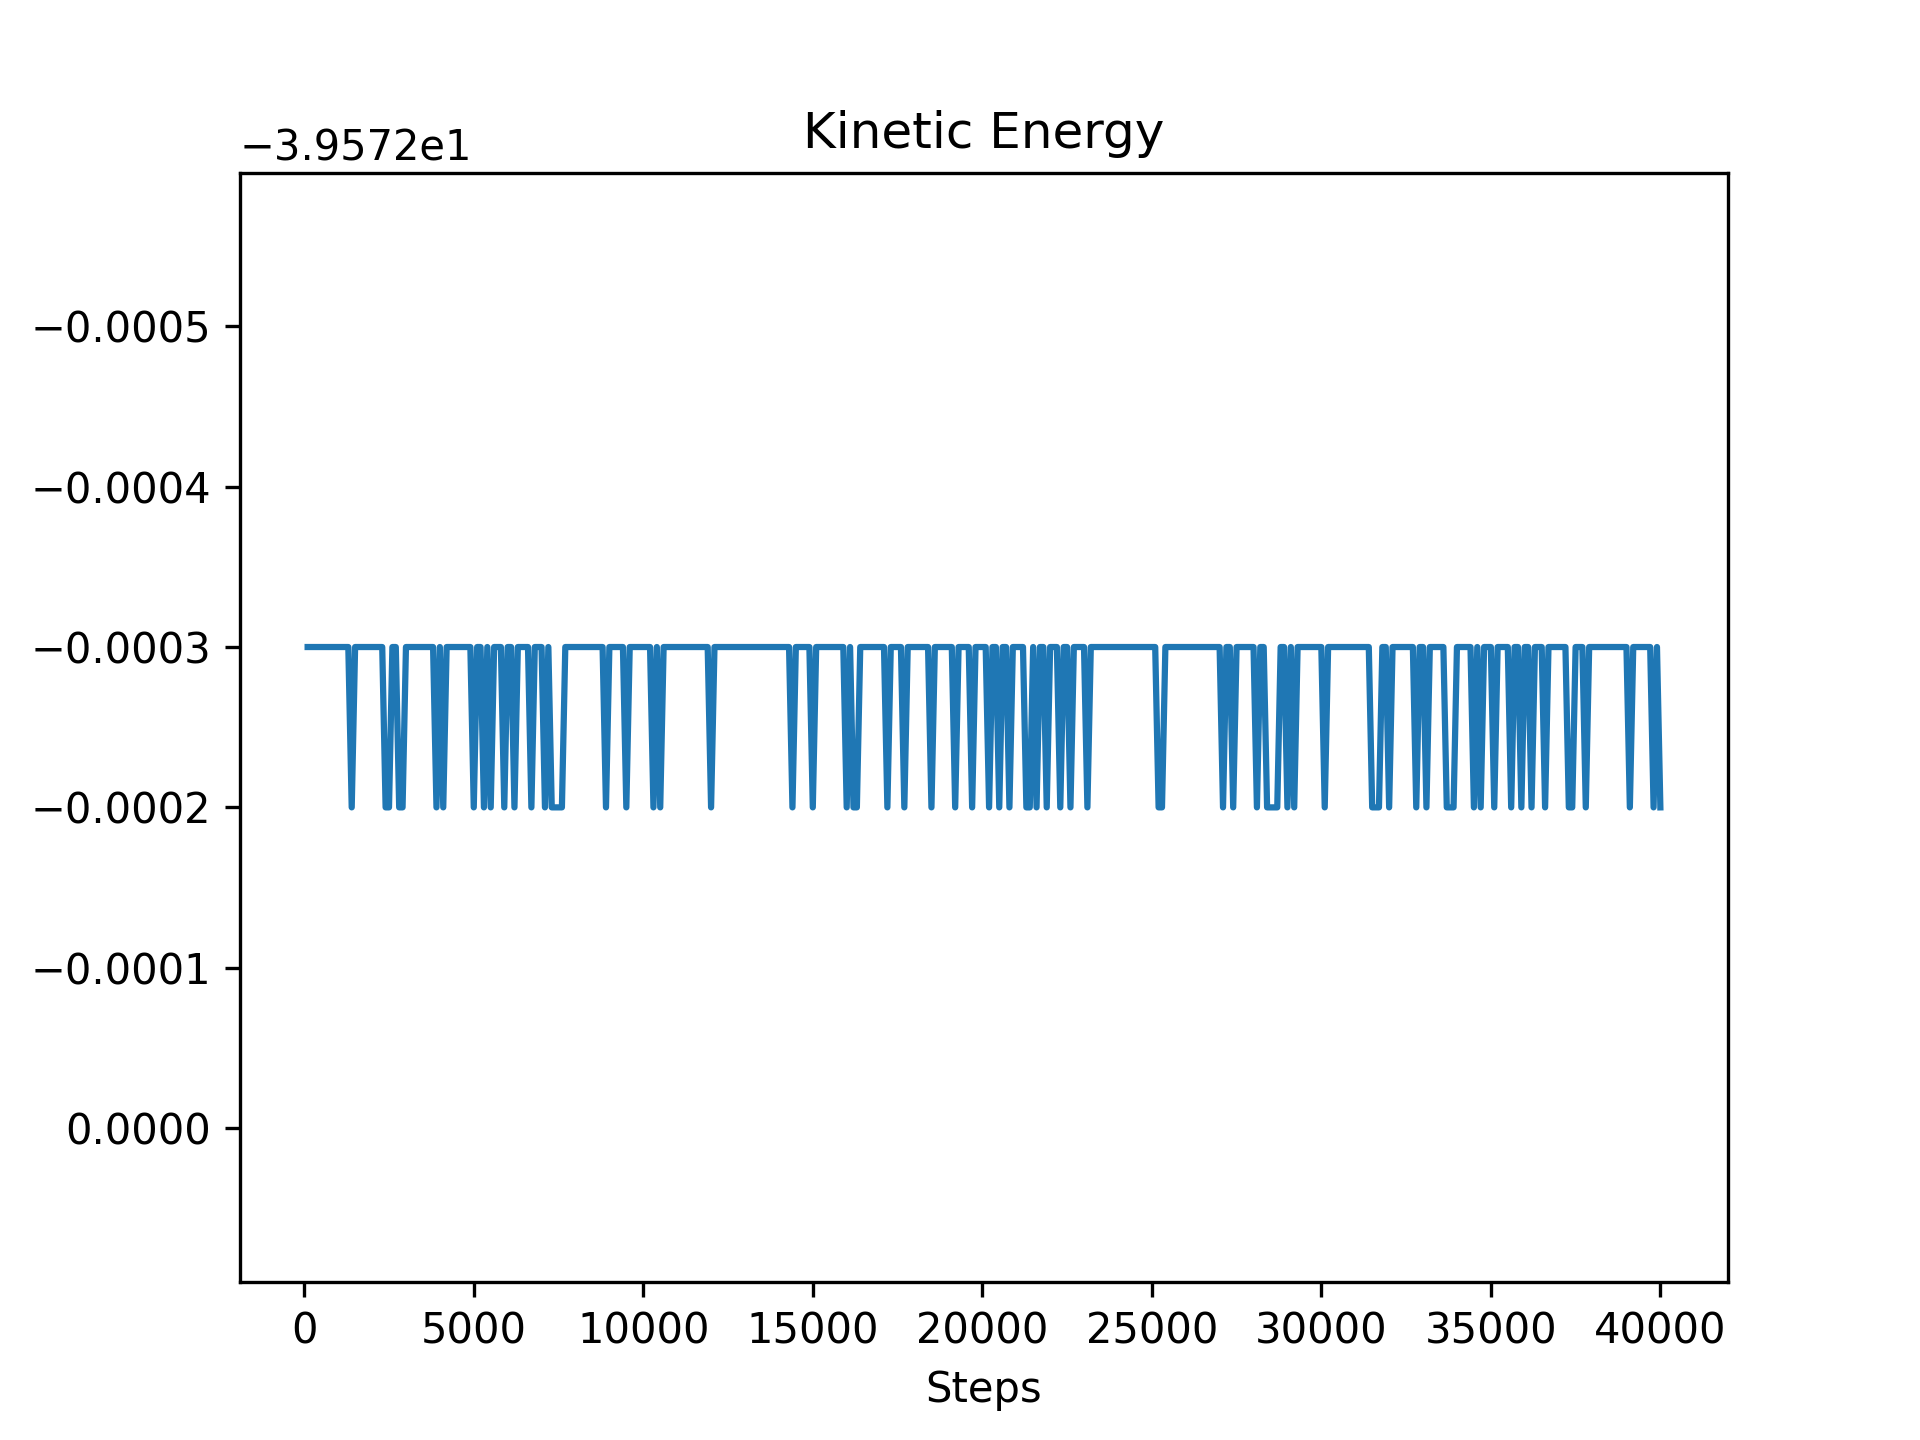
\includegraphics[scale=0.50]{energia1.png}
	\caption{Energía Cinetica}.
\end{figure}

El potencial de Lennard-Jones modela la interacción entre átomos de Xenón a
través de una combinación de fuerzas atractivas de van der Waals a largas
distancias y repulsión fuerte a distancias cortas debido a la superposición
de nubes electrónicas. Este potencial tiene un mínimo de energía en una distancia 
de equilibrio, lo que representa la interacción más estable entre los átomos. Para 
el Xenón, su profundidad $\epsilon$ es relativamente alta, debido a su mayor 
polarizabilidad, lo que influye en sus propiedades macroscópicas como su punto 
de ebullición y su estabilidad en fases líquidas.

\begin{figure}[h]
	\centering
	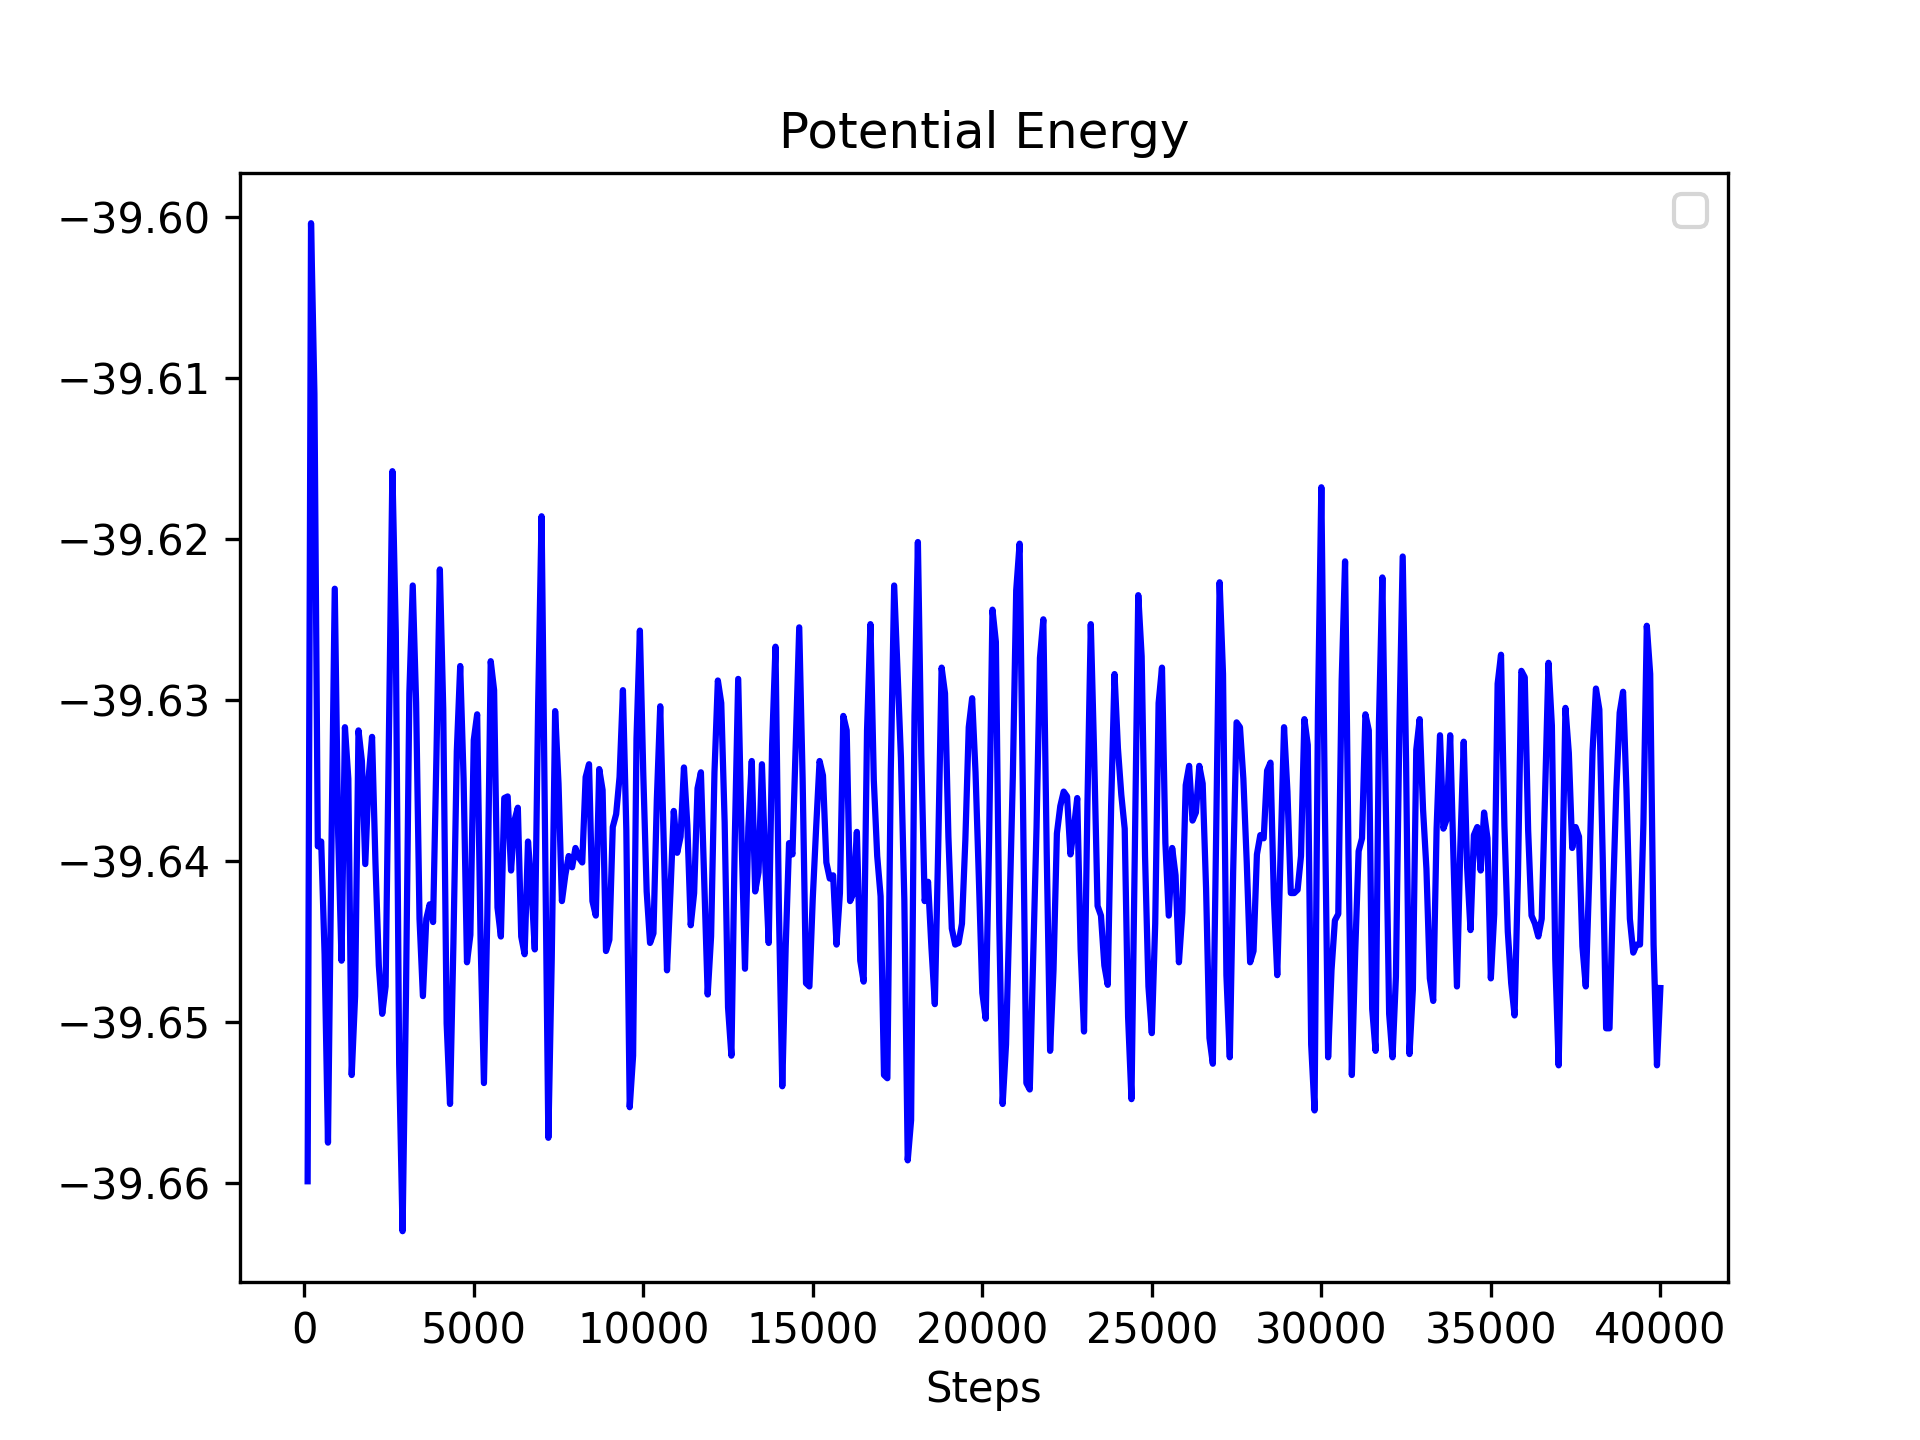
\includegraphics[scale=0.50]{energia2.png}
	\caption{Energía Potencial}.
\end{figure}

La energía total del Xenón refleja el estado energético global del sistema, equilibrando 
el movimiento de los átomos (energía cinética) y sus interacciones intermoleculares 
(energía potencial). Dado que la energía total permanece constante, indica que no hay pérdidas 
ni ganancias de energía externa.

\begin{figure}[h]
	\centering
	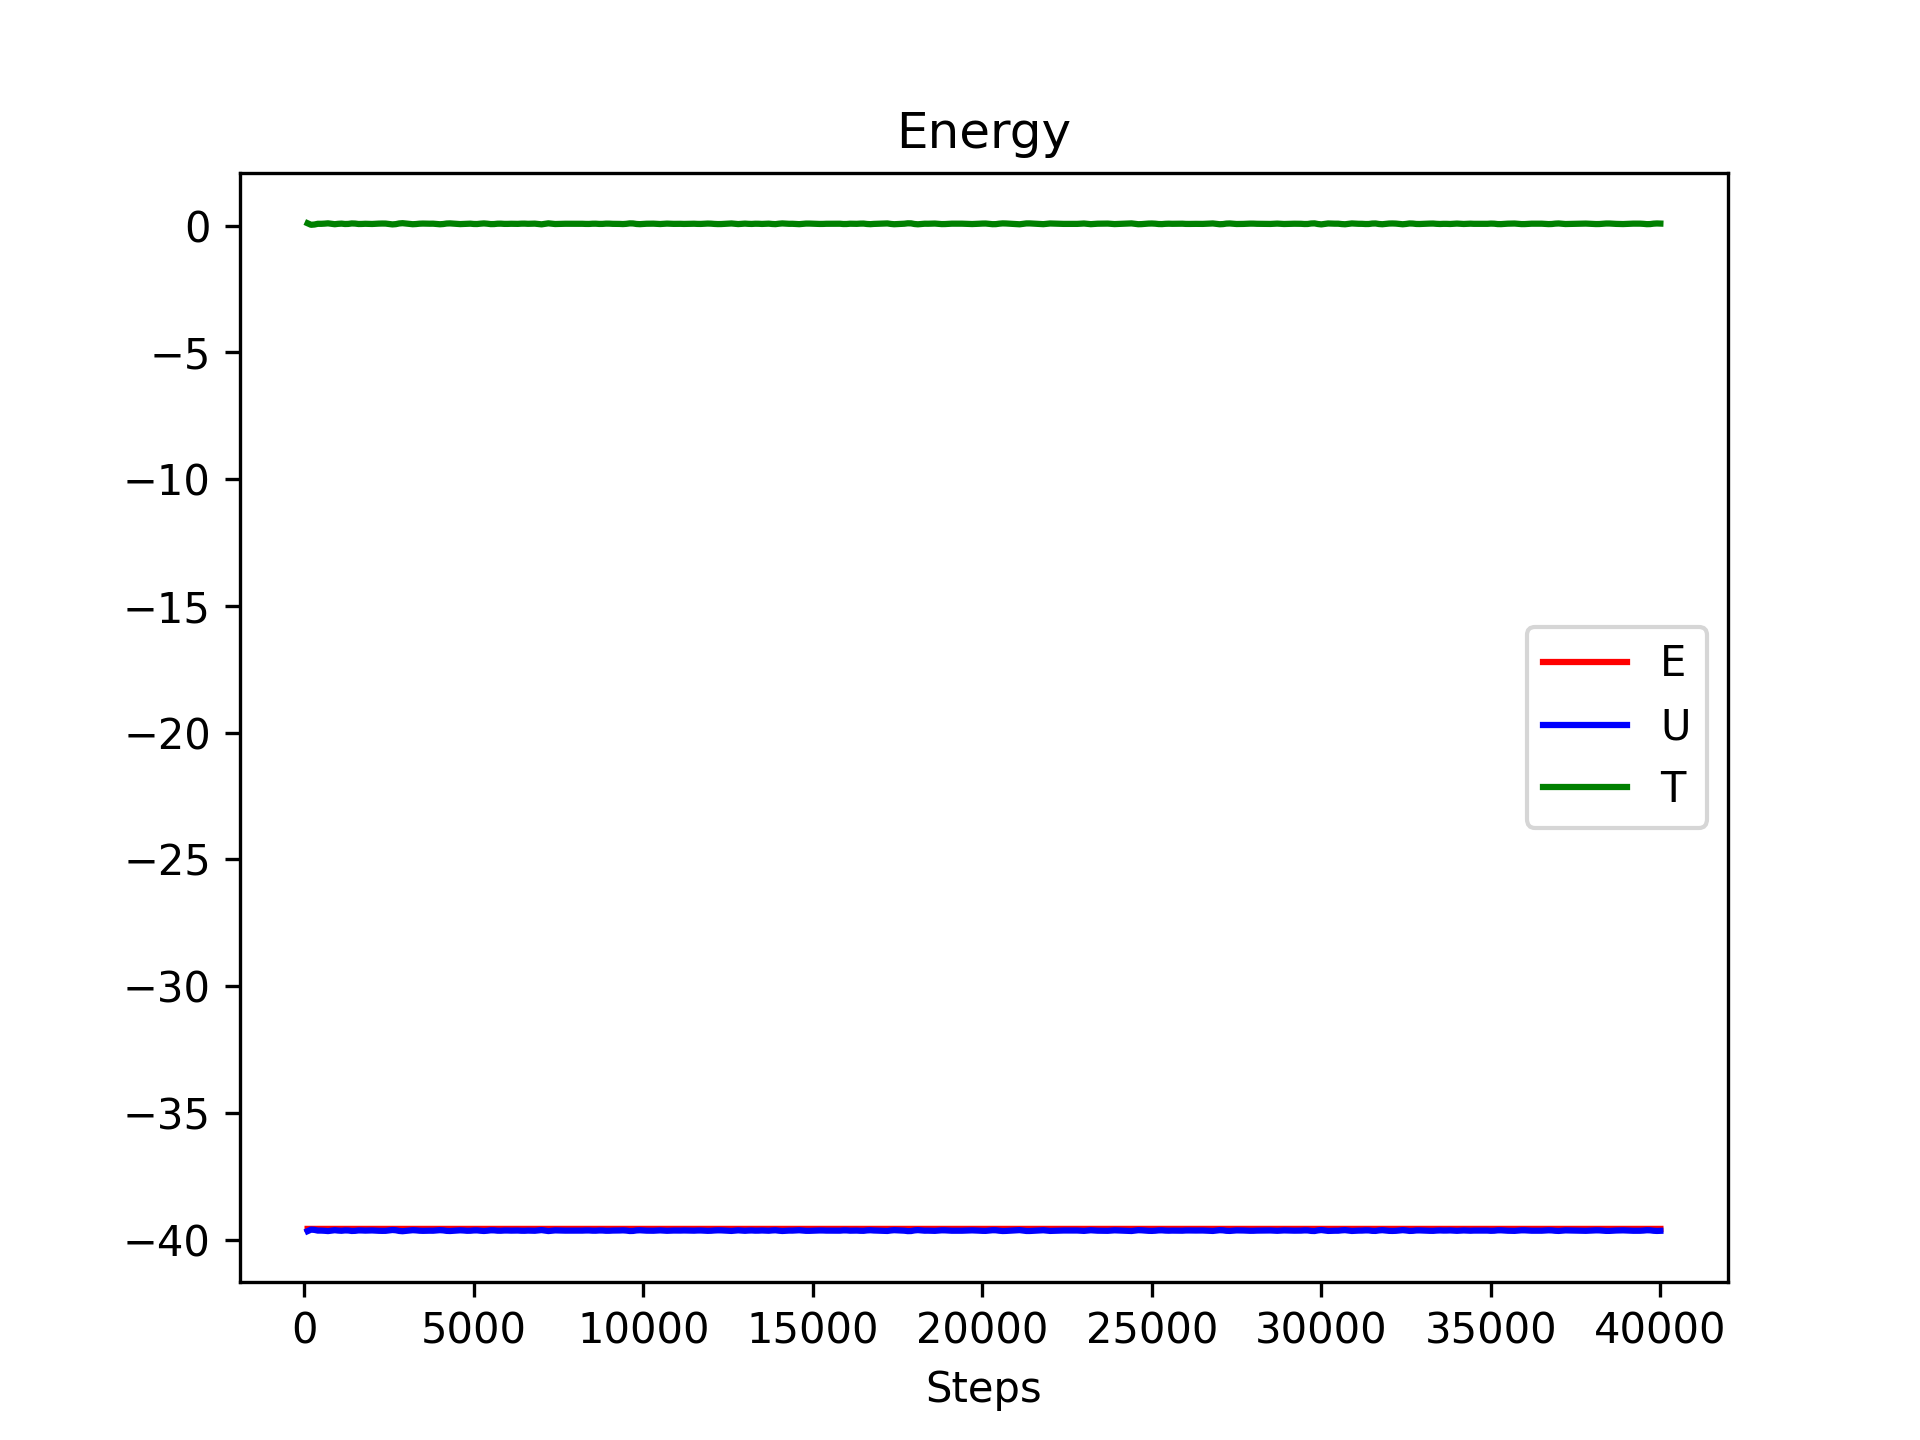
\includegraphics[scale=0.50]{energiat (4).png}
	\caption{Energía Total}.
\end{figure}

\subsubsection*{Temperatura}

A una temperatura promedio de 2K, el sistema ha alcanzado una temperatura extremadamente baja, 
lo que implica que la energía cinética de los átomos de Xenón es mínima. En este rango de 
temperatura, los átomos tienen muy poca energía térmica para moverse, lo que favorece un 
estado sólido o cristalino.

\begin{figure}[h]
	\centering
	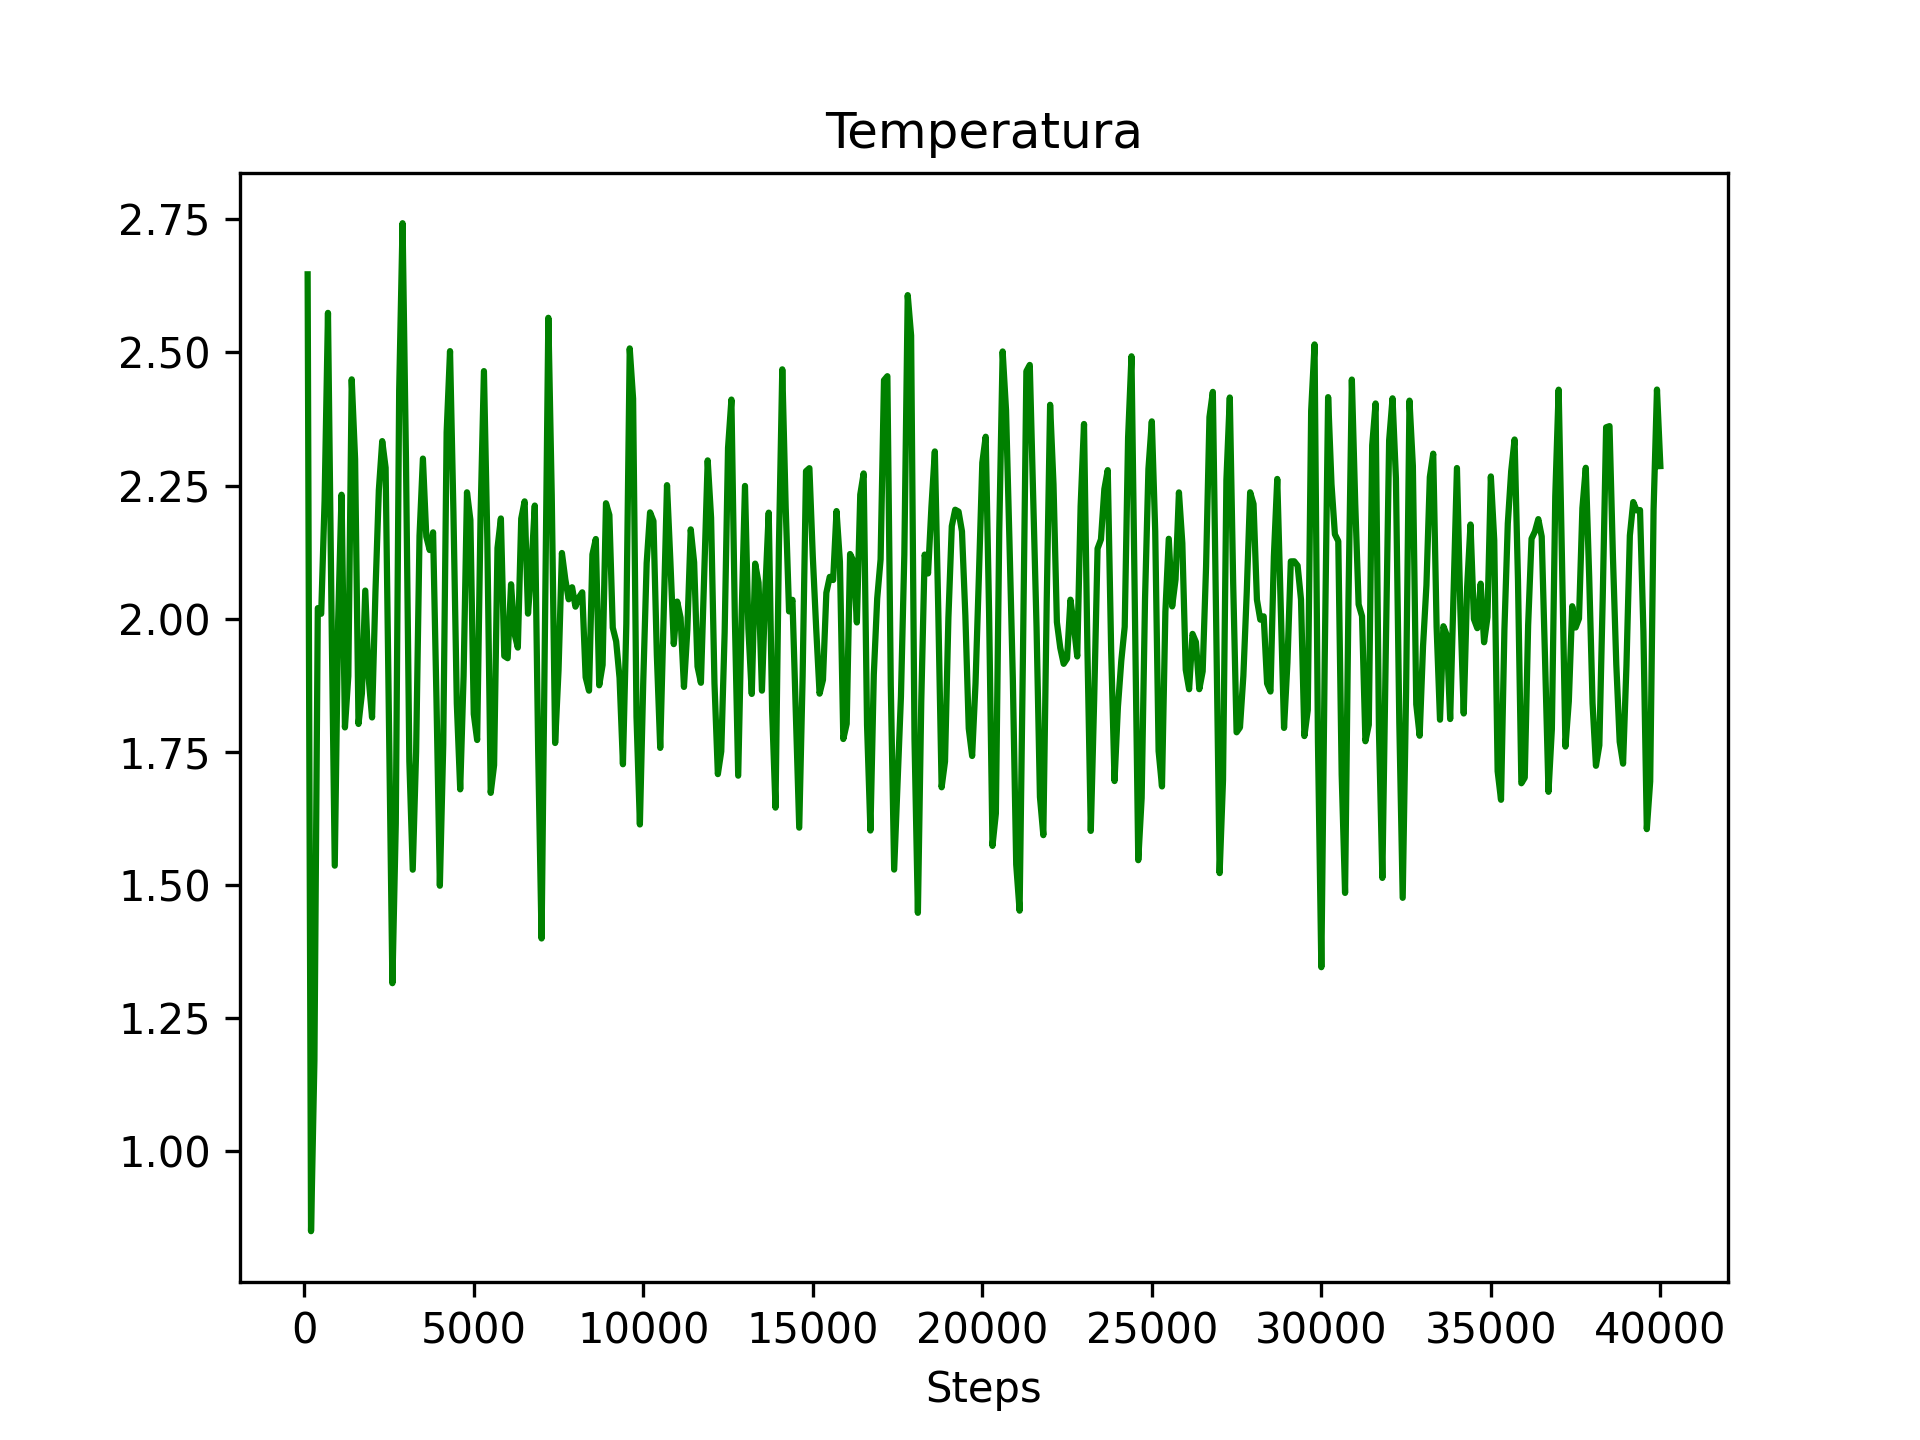
\includegraphics[scale=0.50]{temperatura (3).png}
	\caption{Temperatura}.
\end{figure}

\subsection*{Distribución de pares}

Dado que la geometría del Xenon es FCC, tiene distribuidos 4 átomos en la celda 
unitaria. los peaks más altas son los átomos centrados en la cara, eso quiere decir 
que tiene una mayor concentración de átomos que en sus aristas, los cuales son los 
peaks mas bajos. 

\begin{figure}[h]
	\centering
	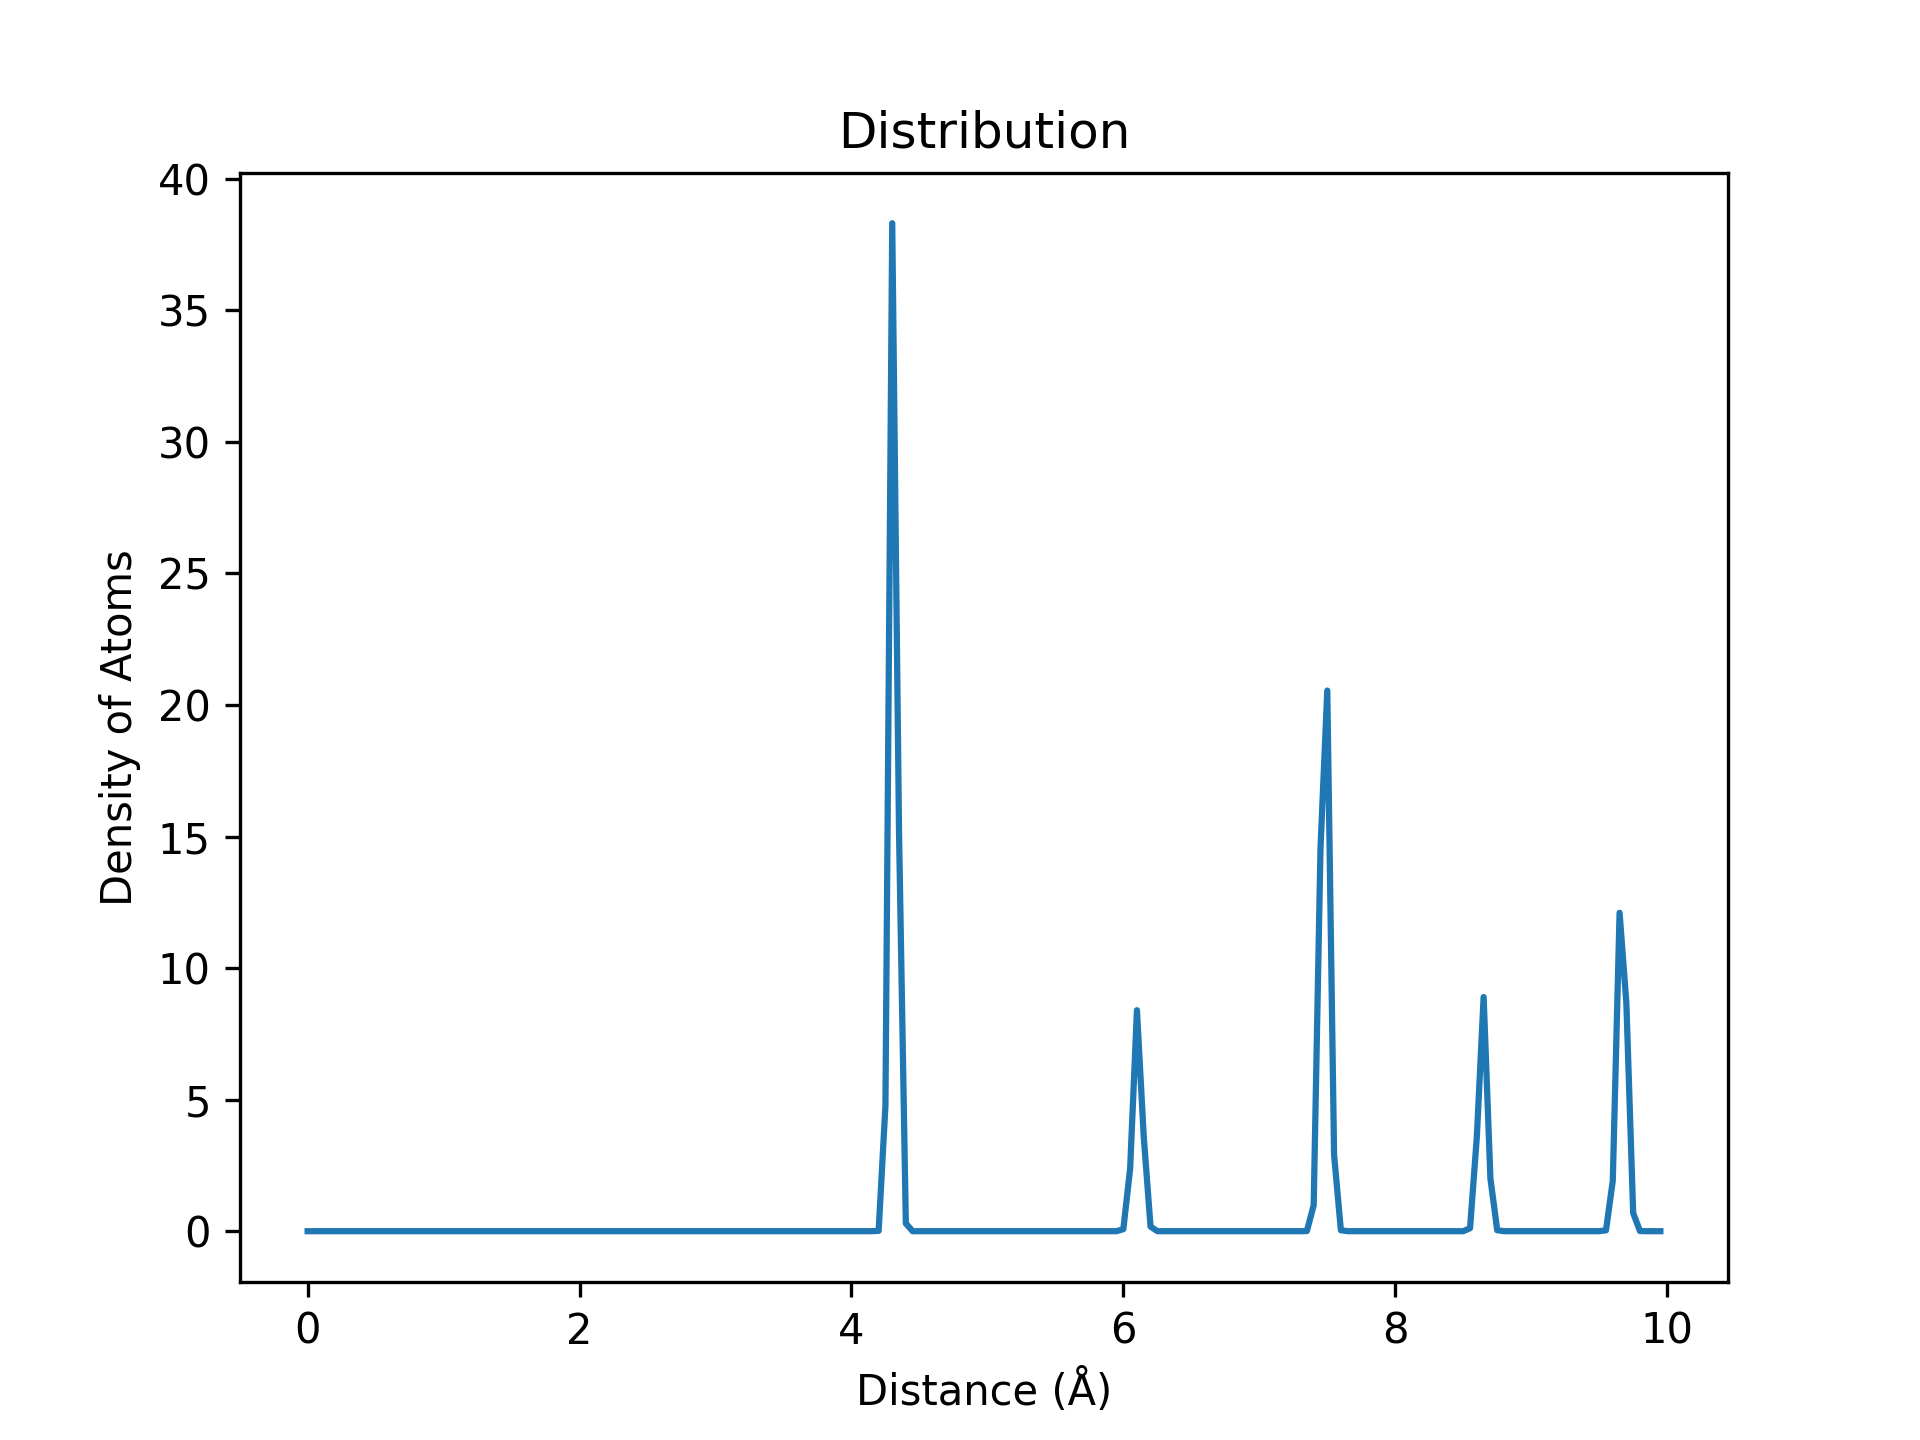
\includegraphics[scale=0.50]{distribution (1).png}
	\caption{Temperatura}.
\end{figure}

\subsection*{Numero de Coordinación}

Tambien llamado ligancia de un átomo central en una molecula o cristal, es el número 
de átomos, moléculas o iones unidos a él.

\begin{figure}[h]
	\centering
	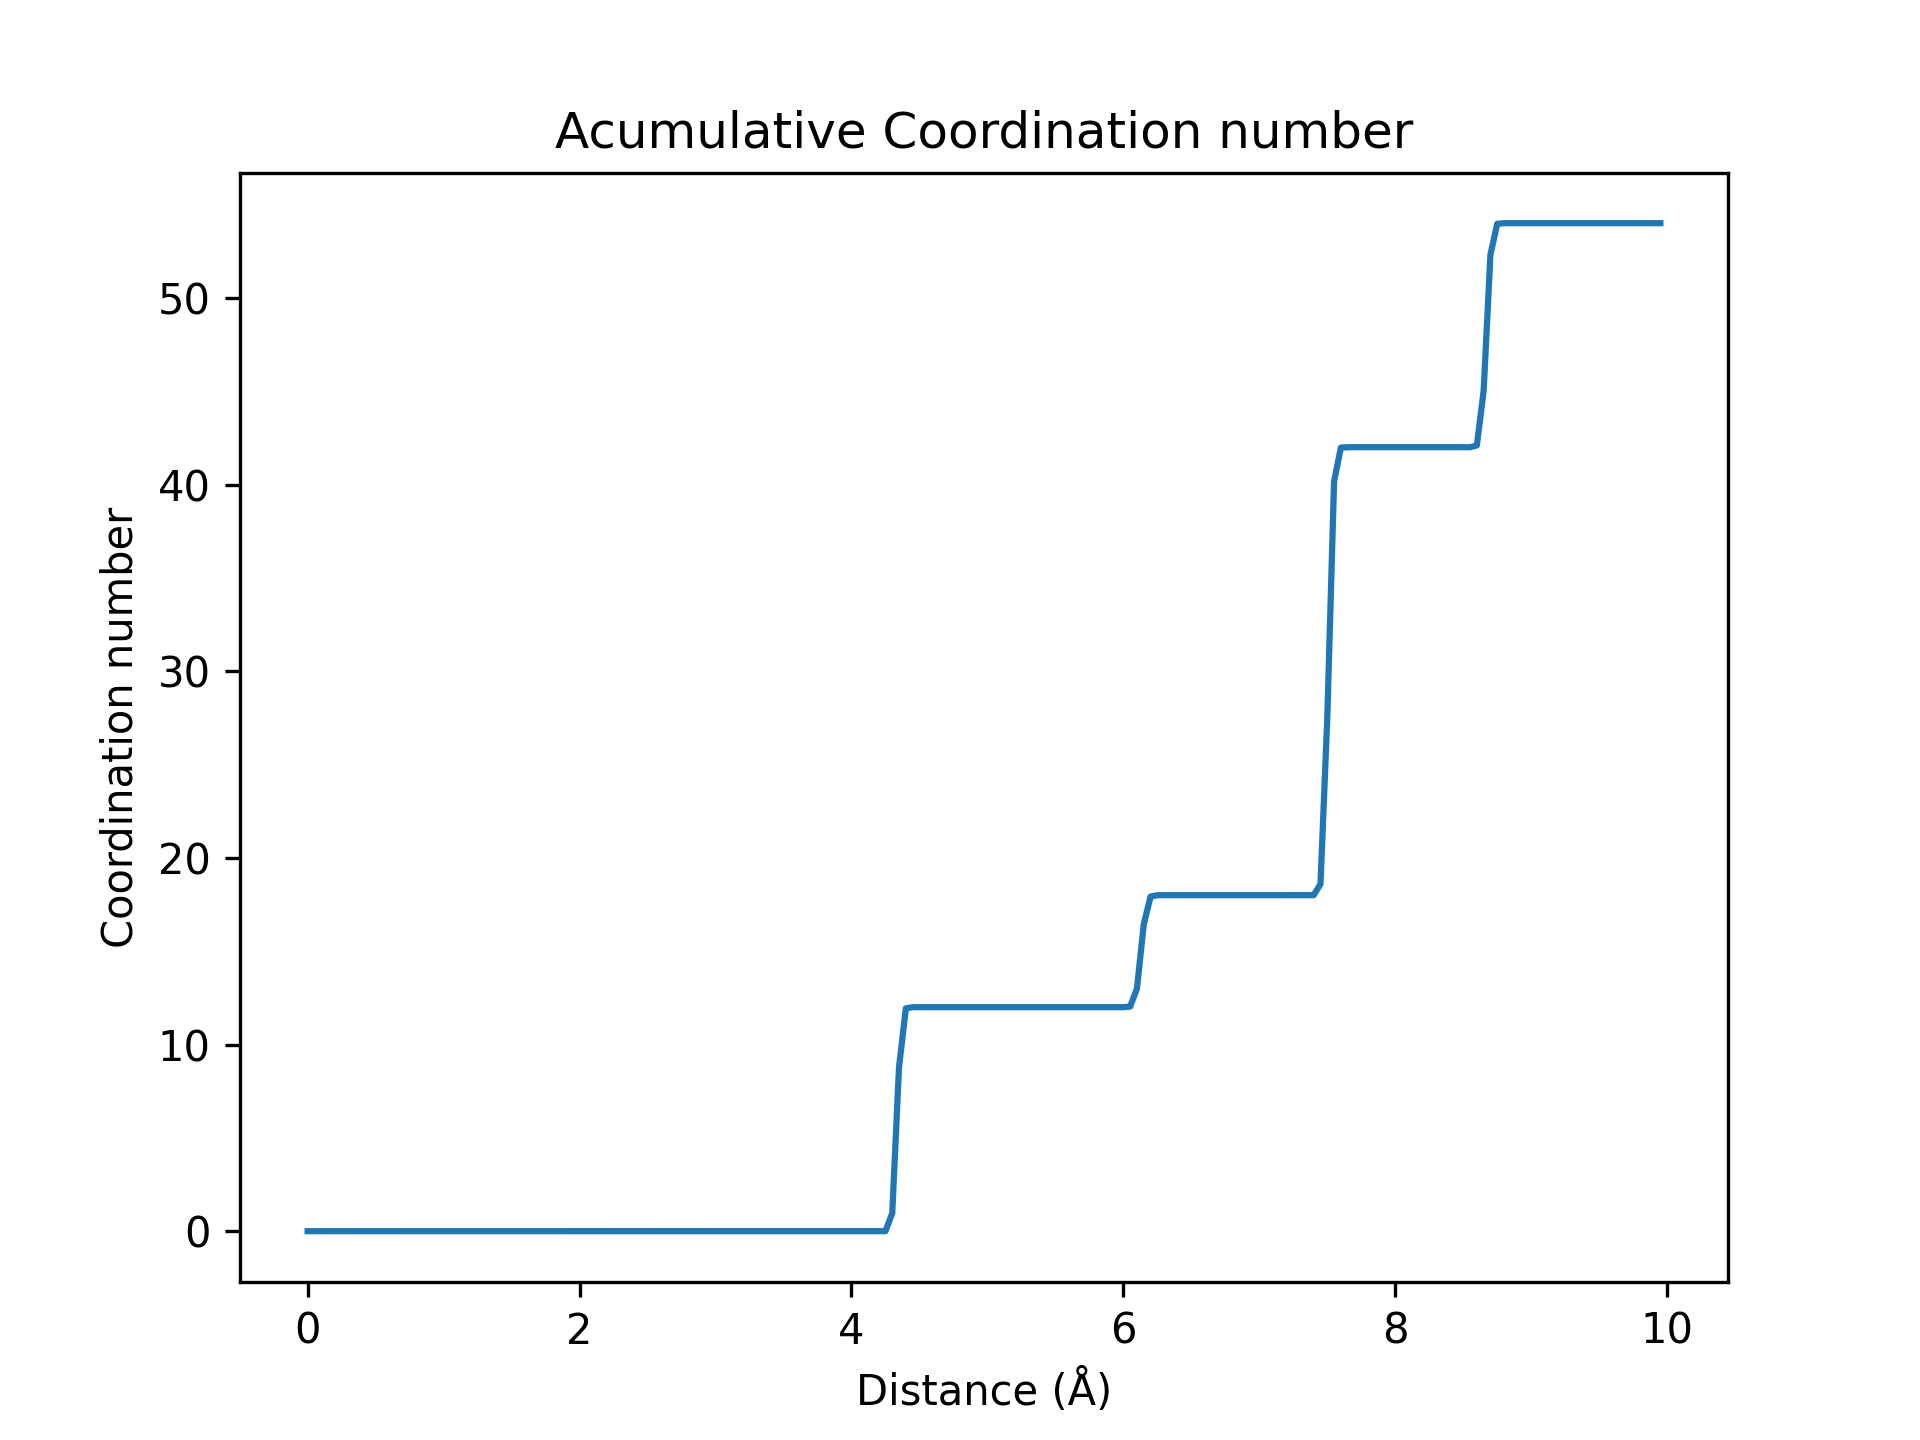
\includegraphics[scale=0.50]{coordination number (1).png}
	\caption{Numero de coordinación acumulativa}.
\end{figure}

En cuyo caso tiene 12 primeros vecinos a una distancia $d_{1}$, 6 a una distancia 
$d_{2}$ y 24 a una distancia $d_{3}$, las cuales fueron descritas anteriormente.

\subsection*{Conclusión}

Podemos concluir que es un ensamble microcanónico como la energía total 
es constante. Internamente la energía cinética y potencial varian, ya que las 
partículas pueden intercambiar energía entre ellas debido a colisiones 
o interacciones. Además el numero de coordinaciones nos confirma que el Xenon 
tiene una estructura fcc, dado que a la distancia $d_{1}$ tiene 12 vecinos.


\end{document}

